	Un garage propose 2 options au client :

	\begin{itemize}[label=\textbullet]
	\item Option Achat : prix d'achat de la voiture $22400 $~\euro{}. Assurance obligatoire $75 $~\euro{} par mois.
	\item Option Location : $425 $~\euro{} par mois, assurance comprise.
	\end{itemize}

	L'objectif de cet exercice est de comparer ces deux options.

	\subsection*{Partie A}

	\begin{enumerate}
		\item Montrer qu'avec l'option Achat la dépense à la fin de la première année est de $\np{23300}$~\euro{}.

		\item Après 36 mois, calculer l'économie réalisée par le client s'il choisit l'option Location?

		\item Afin de comparer les dépenses correspondantes à ces options le client a réalisé le tableau suivant à l'aide d'un tableur :


		\begin{center}
			\begin{sffamily}
			\begin{tabular}{|l|c|c|c|c|c|c|} \hline
			 & A & B & C & D & E & F \\	\hline
				1 & Nombre de mois & 12 & 24 & 36 & 48 & 60 \\ \hline
				2 & Dépense en € Option Achat & \np{23300} & \np{24200} & \np{25100} & \np{26000} & \np{26900} \\ \hline
				3 & Dépense en € Option Location &  &  &  &  &  \\
				\hline
			\end{tabular}
		\end{sffamily}
		\end{center}

		Quelle formule doit être saisie dans la cellule \textsf{B3} qui, étendue jusqu'à la cellule \textsf{F3}, permet de compléter le tableau ?
	\end{enumerate}

	\subsection*{Partie B}

	On souhaite maintenant modéliser les deux options précédentes par des fonctions.

	On note $x$ la durée écoulée en mois depuis la livraison de la voiture.

	La fonction $g$, permettant de calculer la dépense correspondant à l'option Location, peut s'écrire sous la forme : \quad $g(x)=425 x$.

	\begin{enumerate}[resume*]
		\item Déterminer l'expression de $f(x)$ permettant de calculer la dépense correspondant à l'option Achat.

		\item Sur le graphique de la page suivante, on a tracé les courbes représentatives $C_{f}$ et $C_{g}$ des fonctions $f$ et $g$.

		Par lecture graphique, déterminer à partir de combien de mois, l'option Achat est la plus avantageuse.
	\end{enumerate}

	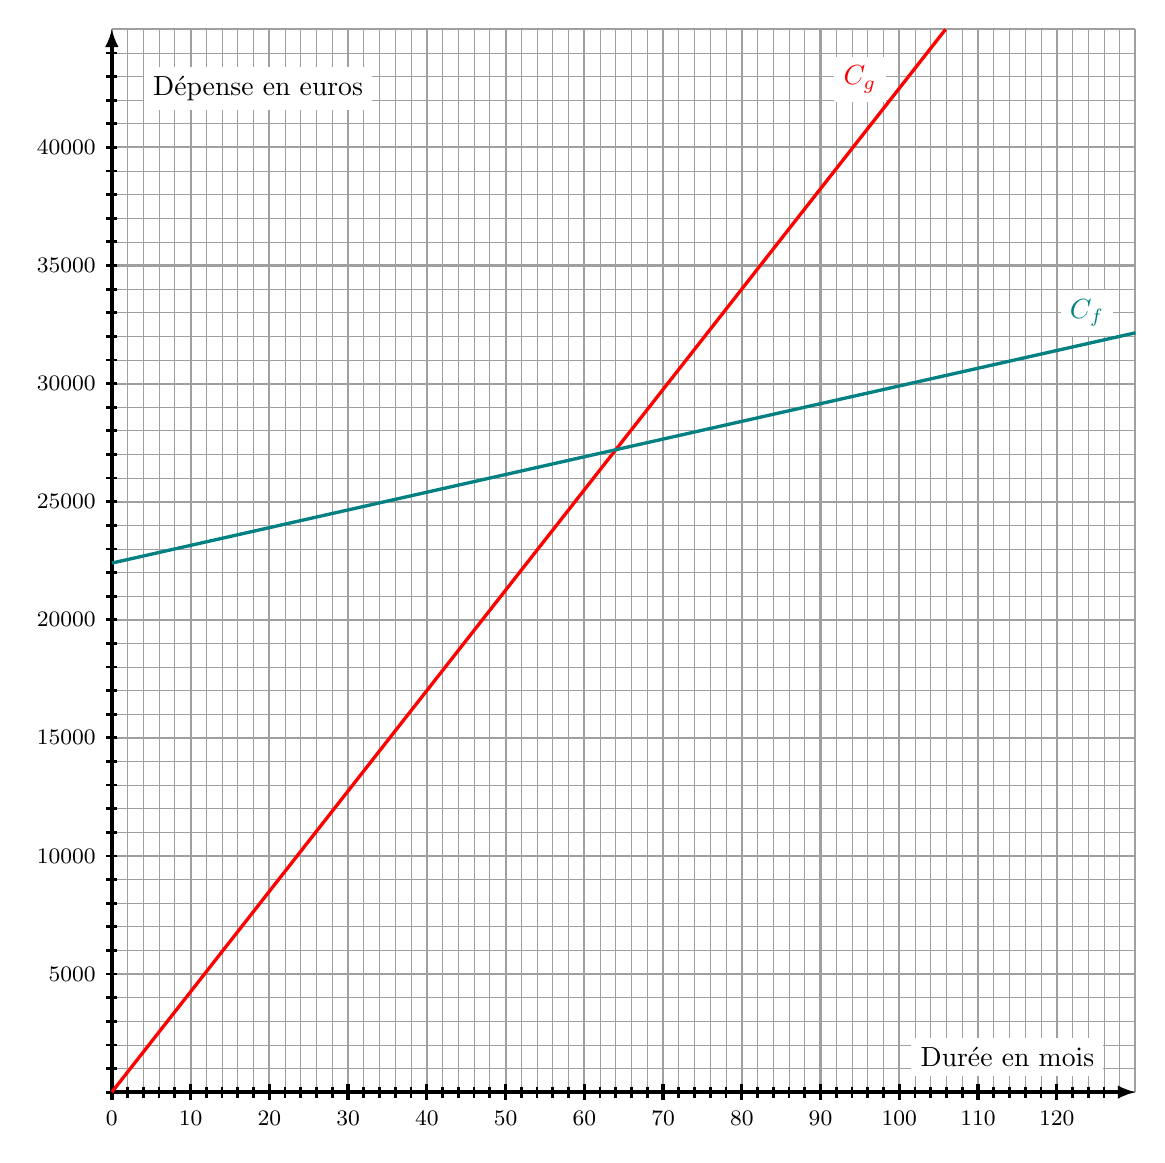
\begin{tikzpicture}[x=1.mm,y=0.03mm,>=latex]%sujet original : x=1.25mm
			\draw [color = gray!75, line width = 0.25pt, xstep=2, ystep = 100] (0,0) grid (130,4500);
			\draw [color = gray!75, line width = 0.75pt, xstep=10, ystep = 500] (0,0) grid (130,4500);
			\draw[<->,line width=1.2pt]
			(0,4500) -- (0,0) -- (130,0);
			\node[left,fill=white] (x) at (126,150){Durée en mois};
			\node[right,fill = white] (y) at (4,4250){Dépense en euros};
			\foreach \x in {0,2,...,126}
			\draw[shift={(\x,0)},color=black,line width=1pt] (0pt,2pt) -- (0pt,-2pt);
			\foreach \x in {0,10,...,120}
			\draw[shift={(\x,0)},color=black,line width=1.2pt] (0pt,3pt) -- (0pt,-3pt) node[below, fill = white] {\footnotesize $\np{\x}$};
			\foreach \y in {0,100,...,4400}
			\draw[color=black,line width=1pt] (2pt,\y) -- (-2pt,\y);
			\foreach \y in {500,1000,...,4000}
			\draw[shift={(0,\y)},color=black,line width=1pt] (2pt,0pt) -- (-2pt,0pt) node[left, fill = white] {\footnotesize $\np{\y0}$};
			\draw[line width=1.2pt,color=red] (0,0)--(1800/17,4500) node[pos=0.93,above left,fill=white]{$C_g$};
			\draw[line width=1.2pt,color=teal] (0,2240)--(130,3215) node[pos=0.98,above left,fill=white]{$C_f$};
	\end{tikzpicture}

